\documentclass{article}
\usepackage[utf8]{inputenc}
\usepackage{fancyhdr}
\usepackage{graphicx}
\usepackage{geometry}
\usepackage{float}

% ---- Commands ------- %
\newcommand{\documentNumber}[1]{
    \LARGE  \textbf{ Kravspecifikation }
    \\
    \medskip
}
\newcommand{\documentVersion}[1]{
    \medskip
}
\newcommand{\documentTitle}[1]{
    \centerline{\rule{13cm}{0.4pt}}
    \bigskip \bigskip
    \LARGE \textbf{Projekt IDA3} \\
    \bigskip
    \LARGE {#1} \\
    \bigskip \bigskip
    \centerline{\rule{13cm}{0.4pt}}
}

\newcommand{\documentDate}[1]{
    \date {#1} 
}


\renewcommand{\arraystretch}{1.7}  % Vertical padding for tables

\renewcommand{\contentsname}{Innehållsförtäckning}

% --- Header & Footer ---- %
\pagestyle{fancy}
\lhead{\leftmark}
\rhead{}
\rfoot{\thepage}
\cfoot{}
\lfoot{}


% ------------------------------------------------ #

% ----- FILL THIS ----- %
\title {
    \documentNumber {01}    

    % Full name - SHORTNAME
    \documentTitle {Helsingborg Event and Convention Bureau}
    
    % Format: YYYY-MM-DD
    \documentDate {2021-08-20}
    \documentVersion Vv 0.1
    
    \author{Anna Bergvall - Oscar Blixt - Pontus Persson - Filip Sjövall - David Vilppu - Sahab Zafar}
}

\begin{document}
\addtocontents{toc}{\protect\setcounter{tocdepth}{2}}
\maketitle

\thispagestyle{empty}



\newpage

\tableofcontents


\newpage

\section{Dokument Historia}
\begin{tabular}{ l | l | l }
    Version & Date & Description \\
    \hline
    0.1 & 2021-10-06 & Dokumentet skapat. \\
    
\end{tabular}

\section{Introduktion}
    Detta dokument representerar kraven för systemet. Systemet är ett frågeformulär vars syfte är att få Helsingborg att bli miljöcertifierad av GDSM. Huvudfunktionaliteten är att HASAB ska kunna sammanställa den data som tillkommit till följd av svar på formuläret från näringslivet. Systemet ska kunna interagera med databas, server och klient.
    

\section{Bakgrund och mål}

    \subsection{Mål}
       Målet är att få Helsingborg stad att bli miljöcertifierad genom att utveckla ett webbaserat frågeformulär som är snabbt och enkelt för användaren att svara på.
        
    \subsection{Viktiga aktörer}
    Systemet kan användas av följande intressenter:
    \begin{enumerate}
        \item \textbf{Slutanvändare:} Slutanvändaren kommer interagera med systemet genom att logga in och svara på de frågor som är relevant för dennes bransch.
        \item \textbf{HASAB:} HASAB ska tilldelas rollen administratör och således ha tillgång till en administrationssida där de kan ta bort, lägga till och redigera frågor och användare.
    \end{enumerate}
    
    \section{Terminologi}
    \begin{enumerate}
        \item \textbf{HASAB:} Förkortning av Helsingborg Arena och Scen AB vilket är företaget som ska utnyttja systemet.
        \item \textbf{Frågeformulär:} Ett webbaserat system som innehåller frågor med flervalsalternativ samt statistikföring över svaren.
        \item \textbf{Administratör:} Administratören har tillgång till systemets alla funktioner.
        \item \textbf{Slutanvändare:}  De personer som svarar på frågeformuläret, vilka främst arbetar inom besöksnäringen i Helsingborgs stad. 
    \end{enumerate}
    
    \section{Stabila krav}
       Stabila krav är krav som inte är ändringbenägna - de baseras på funktioner som är grundläggande för att systemet ska möta beställarens behov. 
    Se scrumboard.
    
    \subsection{Funktionella krav}
    \subsubsection{Krav}
    Systemet ska ha samma gränssnitt som kontextdiagramet visar.
    
    \begin{figure}[h!]
    \caption{Kontext-diagram}
    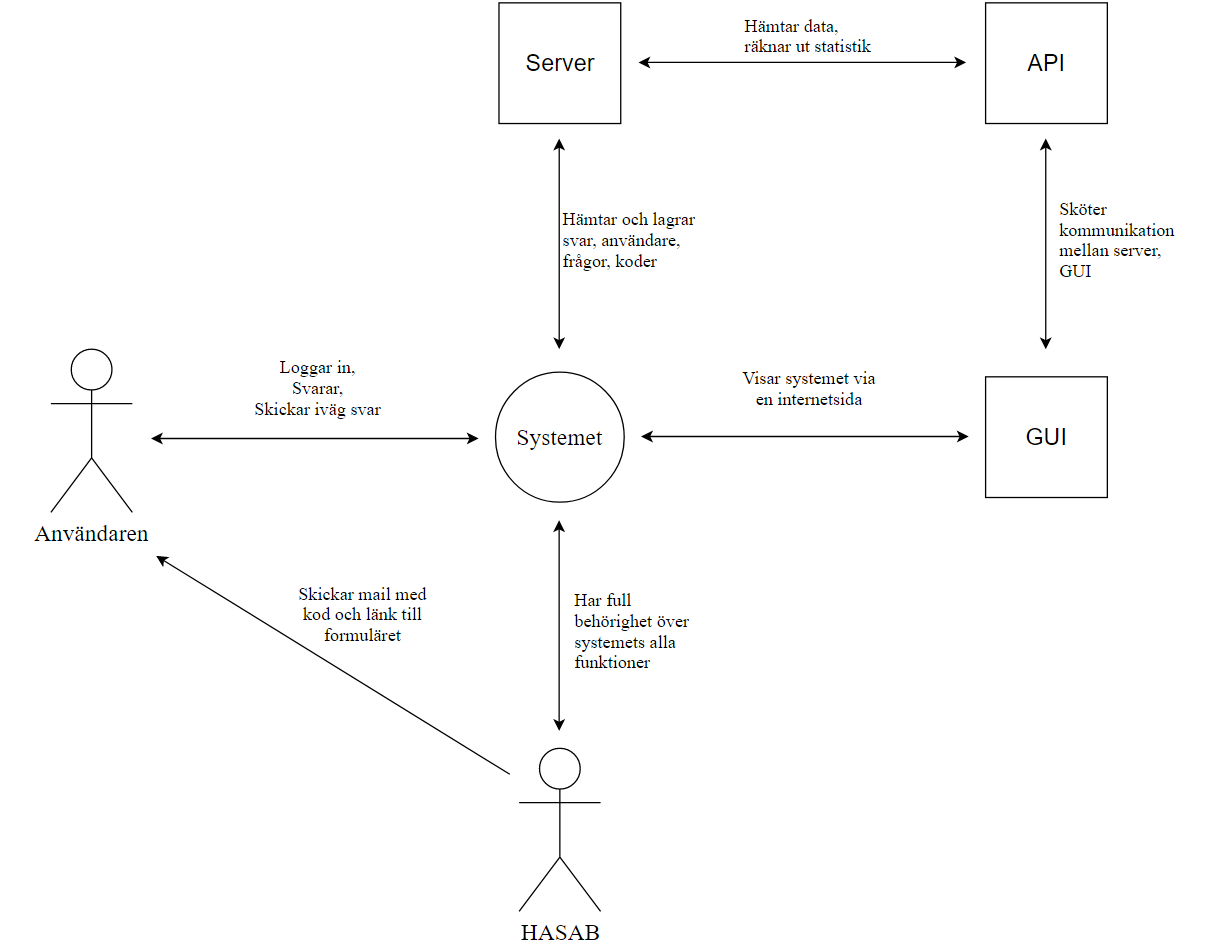
\includegraphics[width=150mm]{Kontextdiagram.png}
    
    \end{figure}
    
    \section{Kvalitetskrav}
    \subsubsection{Prestanda}
    
    \subsubsection{Säkerhet}
    
    \subsubsection{Användbarhet}
    
    \section{Ändringsbenägna krav}
    Krav som är listade här kan förändras eller tas bort.
    
    \begin{figure}[h!]
    
    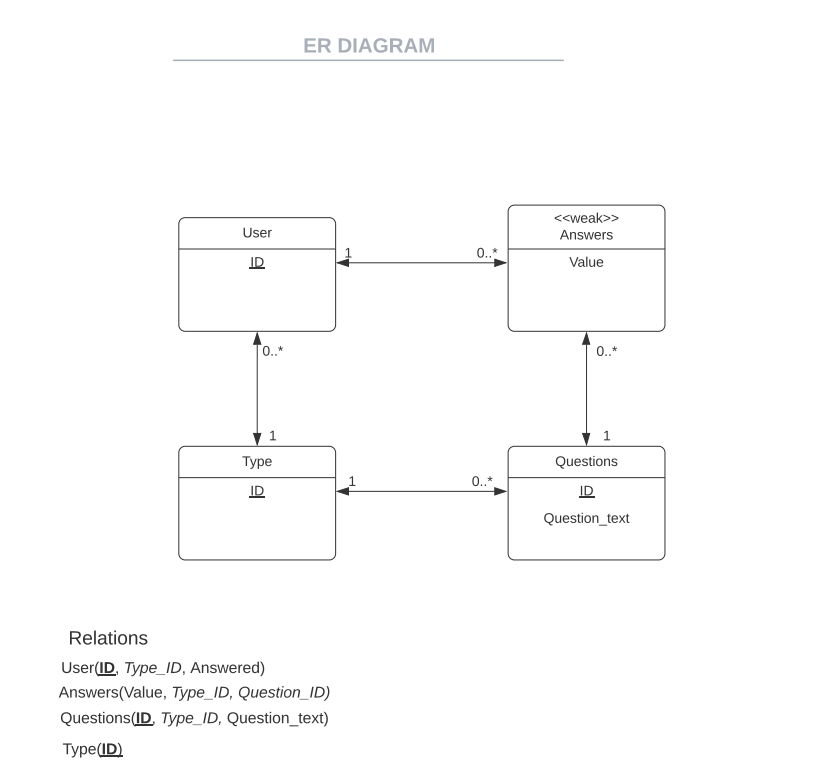
\includegraphics[width=150mm]{ERDIAGRAM.png}
    \caption{ER-Diagram}
    \end{figure}
    
    \section{Uteslutna krav}
    Krav som är listade här är inte längre aktuella.
    
    

    
        




\bibliographystyle{alpha}


\end{document}